%%%%%%%%%%%%%%%%%%%%%%%%%%%%%%%%%%%%%%%%%
% Short Sectioned Assignment LaTeX Template Version 1.0 (5/5/12)
% This template has been downloaded from: http://www.LaTeXTemplates.com
% Original author:  Frits Wenneker (http://www.howtotex.com)
% License: CC BY-NC-SA 3.0 (http://creativecommons.org/licenses/by-nc-sa/3.0/)
%%%%%%%%%%%%%%%%%%%%%%%%%%%%%%%%%%%%%%%%%

%----------------------------------------------------------------------------------------
%	PACKAGES AND OTHER DOCUMENT CONFIGURATIONS
%----------------------------------------------------------------------------------------

\documentclass[paper=a4, fontsize=11pt]{scrartcl} % A4 paper and 11pt font size

% ---- Entrada y salida de texto -----

\usepackage[T1]{fontenc} % Use 8-bit encoding that has 256 glyphs
\usepackage[utf8]{inputenc}
%\usepackage{fourier} % Use the Adobe Utopia font for the document - comment this line to return to the LaTeX default

\usepackage{eurosym}
\usepackage{multirow}
% ---- Idioma --------

\usepackage[spanish, es-tabla]{babel} % Selecciona el español para palabras introducidas automáticamente, p.ej. "septiembre" en la fecha y especifica que se use la palabra Tabla en vez de Cuadro

% ---- Otros paquetes ----

\usepackage{url} % ,href} %para incluir URLs e hipervínculos dentro del texto (aunque hay que instalar href)
\usepackage{amsmath,amsfonts,amsthm} % Math packages
%\usepackage{graphics,graphicx, floatrow} %para incluir imágenes y notas en las imágenes
\usepackage{graphics,graphicx, float} %para incluir imágenes y colocarlas

% Para hacer tablas comlejas
%\usepackage{multirow}
%\usepackage{threeparttable}

%\usepackage{sectsty} % Allows customizing section commands
%\allsectionsfont{\centering \normalfont\scshape} % Make all sections centered, the default font and small caps

\usepackage{fancyhdr} % Custom headers and footers
\pagestyle{fancyplain} % Makes all pages in the document conform to the custom headers and footers
\fancyhead{} % No page header - if you want one, create it in the same way as the footers below
\fancyfoot[L]{} % Empty left footer
\fancyfoot[C]{} % Empty center footer
\fancyfoot[R]{\thepage} % Page numbering for right footer
\renewcommand{\headrulewidth}{0pt} % Remove header underlines
\renewcommand{\footrulewidth}{0pt} % Remove footer underlines
\setlength{\headheight}{13.6pt} % Customize the height of the header

\numberwithin{equation}{section} % Number equations within sections (i.e. 1.1, 1.2, 2.1, 2.2 instead of 1, 2, 3, 4)
\numberwithin{figure}{section} % Number figures within sections (i.e. 1.1, 1.2, 2.1, 2.2 instead of 1, 2, 3, 4)
\numberwithin{table}{section} % Number tables within sections (i.e. 1.1, 1.2, 2.1, 2.2 instead of 1, 2, 3, 4)

\setlength\parindent{0pt} % Removes all indentation from paragraphs - comment this line for an assignment with lots of text

\newcommand{\horrule}[1]{\rule{\linewidth}{#1}} % Create horizontal rule command with 1 argument of height



%----------------------------------------------------------------------------------------
%	TÍTULO Y DATOS DEL ALUMNO
%----------------------------------------------------------------------------------------

\title{	
\normalfont \normalsize 
\textsc{\textbf{Modelos de Computación (2016-2017)} \\ Grado en Ingeniería Informática \\ Universidad de Granada} \\ [25pt] % Your university, school and/or department name(s)
\horrule{0.5pt} \\[0.4cm] % Thin top horizontal rule
\huge Prácticas \\ % The assignment title
\horrule{2pt} \\[0.5cm] % Thick bottom horizontal rule
}

\author{David Criado Ramón} % Nombre y apellidos
\date{}

%----------------------------------------------------------------------------------------
% DOCUMENTO
%----------------------------------------------------------------------------------------

\begin{document}

\maketitle % Muestra el Título

\newpage %inserta un salto de página

\tableofcontents % para generar el índice de contenidos

\newpage
\section{Demostrar que la siguiente gramática genera todas las cadenas formadas por a y b con mismo número de símbolos terminales a que de símbolos terminales b.}
\textbf{G = (V,T,P,S)}, \textbf{V = \{S,A,B\}}, \textbf {T = \{a,b,\}}, donde \textbf{P} es el conjunto de las siguientes reglas de producción: \newline

\begin{table}[H]
	\centering
	\begin{tabular}{cccc}
		\textbf{S -\textgreater\space aB}  & \textbf{S -\textgreater\space bA} & \textbf{A -\textgreater\space a}  & \textbf{A -\textgreater\space aS}  \\
		\textbf{A -\textgreater\space bAA} & \textbf{B -\textgreater\space b}  & \textbf{B -\textgreater\space bS} & \textbf{B -\textgreater\space aBB}
	\end{tabular}
\end{table}

Para demostrarlo dividimos el proceso en dos partes:
\subsection{Demostrar que generamos sólo cadenas que verifican la propiedad dada.}

Para resolverlo vamos a intentar ver la interpretación que cada una de las variables de la gramática. Puesto que el objetivo es obtener cadenas que tengan el mismo número de letras a que de letras b, suponemos que esta será la interpretación de el símbolo inicial S.\newline

Si observamos las producciones que parten de la variable A, vemos que podemos o cambiarlo por el símbolo terminal a, por un símbolo terminal a junto a la variable inicial S, o por un símbolo terminal b junto a dos variables A. Si nos fijamos, por ejemplo, en el símbolo terminal a junto a la variable inicial S observamos que si seguimos la definición que debe de ocurrir para que la propiedad ocurra una variable A genera una cadena que tiene exactamente un símbolo terminal a más que el número de símbolos terminales b. Ahora comprobemos que esta supuesta interpretación es correcta en los otros dos casos, en el que la variable A pasa al símbolo terminal a es evidente que hay un símbolo más a (1) que b (0), y en el que la variable A pasa al símbolo b junto a dos variables A, debido a la interpretación que hemos dado sabemos que las variables A producirán siempre una a más que b, así pues, al añadir dos variables A en la parte derecha es necesario que también aparezca el símbolo terminal b para cumplir la interpretación.\newline

En el caso de la variable B, podemos observar que las producciones son idénticas a las de la variable A intercambiando los símbolos terminales y cambiando las variables A por B.\newline

Puesto que del símbolo inicial sólo podemos generar una cadena que empiece por a y símbolo terminal B (que garantizará que cuando se desarrolle la B habrá un símbolo terminal b más que a), o ir del símbolo inicial al caso análogo (empezar por b seguida de símbolo terminal A) podemos verificar que se generan sólo las cadenas deseadas.
\subsection{Demostrar que generamos todas las cadenas que verifican la propiedad dada.}
Para demostrarlo hemos de ver todas las líneas de derivación posibles que pueden generar esta gramática y ver que efectivamente es posibles generarlas todas. A partir del símbolo inicial S siempre podemos generar o una la cadena aB o la cadena Ba. Si consideramos la cadena aB, para poder generar todas las cosas a partir de la variable B necesitamos:
\begin{itemize}
	\item Acabar con una única b para equilibrar el número de a y de b disponibles (S ->\space aB, B ->\space b, ab).
	\item Añadir la b y dar posibilidad de continuar con una a (S ->\space aB, B ->\space bS, abS, S ->\space aB, abaB, etc...).
	\item Añadir una b y dar posibilidad de continuar con otra b (S ->\space aB, B->\space bS, abS, S->\space bA, abbA, etc...).
	\item Añadir una a y poder continuar con otra a (S ->\space aB, B ->\space aBB, aaBB, B->\space aBB, aaaBBB, etc...).
	\item Añadir una a y poder continuar con una b (S ->\space aB, B ->\space aBB, aaBB B -> \space b, aabB, etc...).
\end{itemize}

Puesto que los casos a partir de la variable B, son análogos a partir de la variable A, podemos afirmar que se pueden generar todas las cadenas con el criterio dado.

\section{Determinar si la siguiente gramática genera un lenguaje regular (tipo 3).}

Gramática libre del contexto \textbf{G = (V,T,P,S)}, \textbf{V = \{S,A,B\}}, \textbf {T = \{a,b,c,d\}}, donde \textbf{P} es el conjunto de las siguientes reglas de producción: \newline

\begin{table}[H]
	\centering
	\begin{tabular}{lcc}
		\textbf{S -\textgreater \space AB}                     & \textbf{A -\textgreater \space Ab} & \textbf{A -\textgreater \space a} \\
		\multicolumn{1}{c}{\textbf{B -\textgreater \space cB}} & \textbf{B -\textgreater \space d}  & \textbf{}                 
	\end{tabular}
\end{table}

Para determinar si la gramática genera un lenguaje regular dividimos el proceso en dos partes:

\subsection{Determinar el lenguaje que es generado la gramática}
Para ello miramos lo podemos obtener de la líneas de derivación. Partiendo del símbolo inicial S sólo podemos llegar a la cadena AB. \newline 
Partiendo de la variable A, podemos o mantener la variable y añadir un símbolo terminal b todas las veces que queramos (repitiendo la misma producción) o pasar la variable A a un único símbolo terminal a que se encontrará a la izquierda. Por tanto, la cadena empieza con un único símbolo terminal a y  una cantidad indeterminada (se admite 0), \textit{i}, de letras b. \newline

Partiendo de la variable B, podemos o añadir un número indeterminado, \textit{j}, de letras c y mantener la variable (repitiendo la misma producción) o pasar la variable B a un única d, por tanto, podemos determinar que el lenguaje generador por la gramática proporcionada es \textbf{$\{L = ab^{i}c^{j}d : i, j \in \mathbb{N} \}$}

\subsection{¿Podemos encontrar una gramática regular que genere el lenguaje?}
Puesto que es necesario que la cadena inicial podemos añadir una producción que nos permita añadir la a y una variable para continuar con el resto de la cadena, por ejemplo, \textbf{S -> \space aB}. La B nos ha de permitir continuar con una serie de símbolos terminales opcionales \textbf{(B -> \space bB)} o pasar a otra v variable C \textbf{(B->C)} que se encargará de añadir todas los símbolos terminales c que queramos \textbf{(C -> \space cC)} o incluso 0 si no usamos esta producción y usamos sólo la que nos permite añadir una d al final a partir de una variable C \textbf{(C -> \space d)}. Por tanto, hemos podido encontrar una gramática regular que genera el mismo lenguaje.

\section{Hacer la máquina de Mealy que decodifica las cadenas generadas por la siguiente máquina:}
\begin{figure}[H]
	\centering
	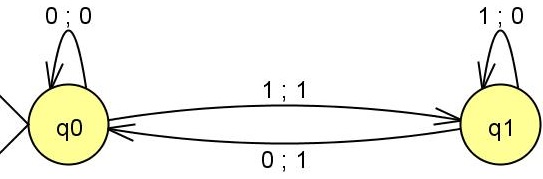
\includegraphics[scale=0.5]{ejer3-codifica.jpg}
	\caption{Máquina de Mealy para la codificación.}
\end{figure}

Para entender cómo la máquina codifica el mensaje hemos de darle una interpretación y ver qué ocurre en cada uno de los casos. Podemos observar que desde el estado q0 ocurre o que bien acabamos de empezar la lectura de la cadena o que lo que hemos leído previamente es un 0. El estado q1 queda determinado por haber leído previamente un 1. Por tanto, para facilitar la visualización de las transiciones voy a organizar los datos en una tabla. 

\begin{table}[H]
	\centering
	\begin{tabular}{|l|l|}
		\hline
		\multicolumn{1}{|c|}{\multirow{2}{*}{Primer símbolo q(0)}} & 0 -\textgreater\space 0 \\ \cline{2-2} 
		\multicolumn{1}{|c|}{}                                     & 1 -\textgreater\space 1 \\ \hline
		\multirow{2}{*}{Anteriormente leído 0 (q0)}                & 0 -\textgreater\space 0 \\ \cline{2-2} 
		& 1 -\textgreater\space 1 \\ \hline
		\multirow{2}{*}{Anteriormente leído 1 (q1)}                & 0 -\textgreater\space 1 \\ \cline{2-2} 
		& 1 -\textgreater\space 0 \\ \hline
	\end{tabular}
	\caption{Tabla de transiciones \textit{(leído -> escrito)} para la máquina de la codificación. }
\end{table}
Para hacer la tabla que decodifique simplemente hemos de invertir cada una de las transiciones de la tabla original, obteniendo por tanto:
\begin{table}[H]
	\centering
	\begin{tabular}{|l|l|}
		\hline
		\multicolumn{1}{|c|}{\multirow{2}{*}{Primer símbolo q(0)}} & 0 -\textgreater\space 0 \\ \cline{2-2} 
		\multicolumn{1}{|c|}{}                                     & 1 -\textgreater\space 1 \\ \hline
		\multirow{2}{*}{Anteriormente leído 0 (q0)}                & 0 -\textgreater\space 0 \\ \cline{2-2} 
		& 1 -\textgreater\space 1 \\ \hline
		\multirow{2}{*}{Anteriormente leído 1 (q1)}                & 1 -\textgreater\space 0 \\ \cline{2-2} 
		& 0 -\textgreater\space 1 \\ \hline
	\end{tabular}
	\caption{Tabla de transiciones \textit{(leído -> escrito)} para la máquina de la decodificación. }
\end{table}

Y siguiendo la representación gráfica del autómata la siguiente:

\begin{figure}[H]
	\centering
	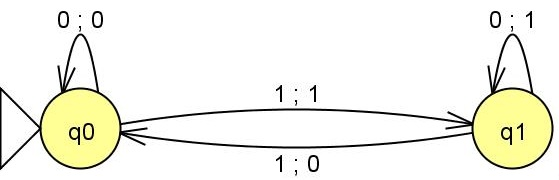
\includegraphics[scale=0.5]{ejer3-decodifica.jpg}
	\caption{Máquina de Mealy para la decodificación.}
\end{figure}

Para comprobar que funciona correctamente vamos a comprobarlo usando JFLAP. Para ello introducimos la cadena de ejemplo 1000101 en la máquina de Mealy que codifica el mensaje y la codificación obtenida la pasamos por la máquina que decodifica tal y como podemos comprobar en la siguientes capturas:

\begin{figure}[H]
	\centering
	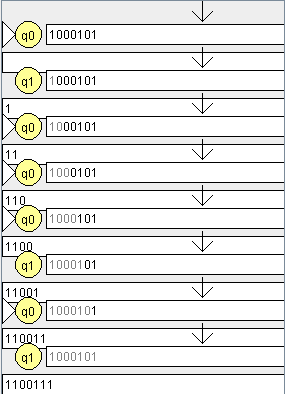
\includegraphics[scale=0.8]{ej-codifica.png}
	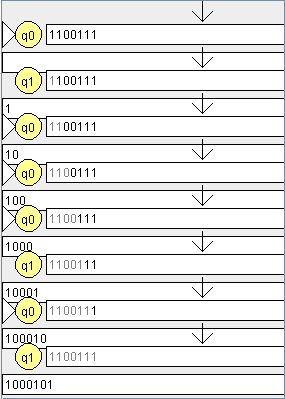
\includegraphics[scale=0.8]{ej-decodifica.png}
	\caption{Procesos de codificación y decodificación de la cadena ejemplo.}
\end{figure}

\section{Ejemplo de uso de LEX}
En esta práctica vamos a probar el uso de lex, en concreto voy a usar flex (fast lex). Para instalarlo sobre kubuntu 16.10 utilizamos el comando \verb|sudo apt-get install flex|.

Vamos a usar el archivo de ejemplo que vemos en el cat de la imagen. En el definimos las expresiones regulares para identificar: conjuntos de letras (no valen letras con tilde), dígitos, signos, sucesiones de dígitos, enteros (combinación de dígitos que pueden tener un signo al principio) y reales (que pueden empezar con signo o no y han de tener una sucesión de dígitos seguida de un punto y otra sucesión de dígitos). Cada vez que se encuentra una ocurrencia de los mismos u combinaciones de ellos es sacada por la salida estándar (como podemos observar en la segunda sección del archivo) y en concreto se suman los enteros para mostrar las ocurrencias de cada tipo (como podemos ver en la tercera sección).

\begin{figure}[H]
	\centering
	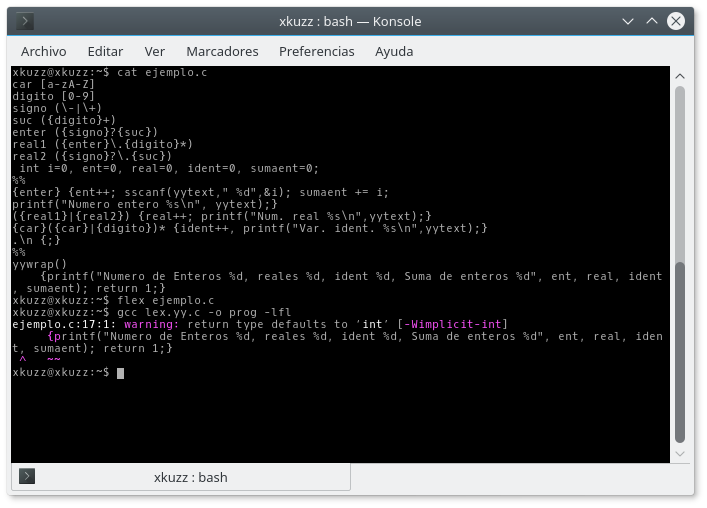
\includegraphics[scale=0.75]{flex1.png}
	\caption{Archivo de ejemplo y comandos de compilación.}
\end{figure}

Para empezar el proceso de compilación ejecutamos el comando flex sobre el archivo en el que hemos escrito las expresiones regulares. La ejecución de flex dará lugar a la creación de un archivo lex.yy.c que será un ejecutable en C y para compilarlo utilizamos gcc linkando con la librería, es decir, utilizamos el comando \verb| gcc lex.yy.c -o prog -lfl|. Por tanto ya sólo nos queda utilizar el programa compilado y redireccionando la entrada y salida estándar a los archivos que deseemos.
\begin{figure}[H]
	\centering
	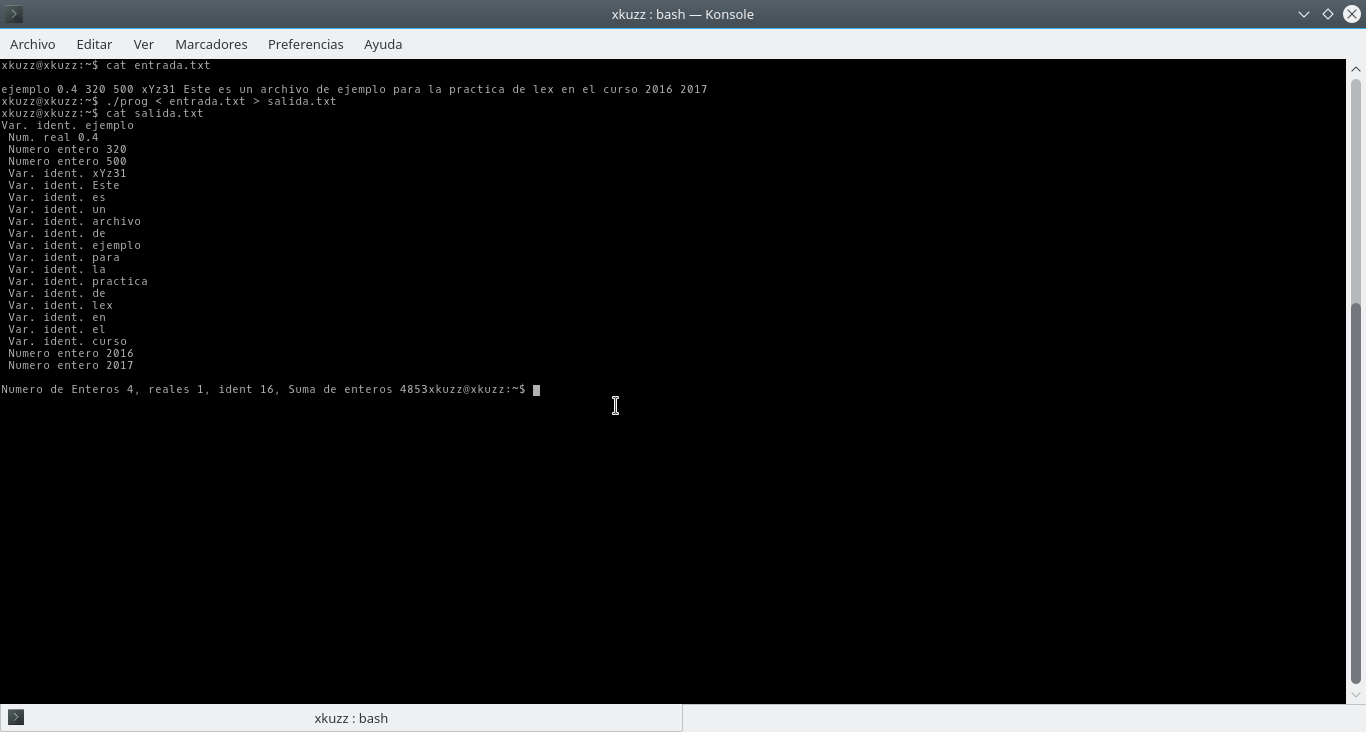
\includegraphics[scale=0.45]{flex2.png}
	\caption{Uso del programa compilado para analizar un archivo de prueba.}
\end{figure}

Si vemos el contenido del archivo de salida vemos como se muestra cada ocurrencia de cada tipo de expresiones regulares y se han contabilizado cuántas habían salido al ejecutar el programa.

\section{Estudiar la ambigüedad generada por la siguiente gramática:}
\textbf{G = (V,T,P,E)}, \textbf{V = \{E,I\}}, \textbf {T = \{a,b,c,d\}}, donde \textbf{P} es el conjunto de las siguientes reglas de producción: \newline

\begin{table}[H]
	\centering
	\begin{tabular}{cccc}
		\textbf{E -\textgreater\space I} & \textbf{E -\textgreater\space I - E} & \textbf{E -\textgreater\space E - I} & \textbf{I -\textgreater\space a|b|c|d}
	\end{tabular}
\end{table}
\subsection{¿Es la gramática ambigua?}
Una gramática es ambigua si para al menos una cadena generada por la gramática puede ser obtenida mediante dos árboles de derivación distintas. Así pues la manera más simple de demostrar que una gramática es ambigua es encontrar dicha cadena que es generada por varios árboles de derivación. En nuestro caso es bastante fácil ver que a - b - c es una cadena generada por los dos siguientes árboles de derivación.

\begin{figure}[H]
	\centering
	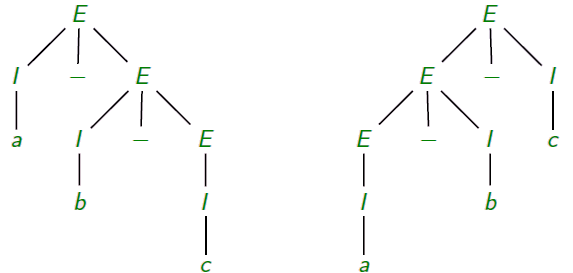
\includegraphics[scale=1.0]{arbol.png}
\end{figure}

\subsection{¿Es el lenguaje inherentemente ambiguo?}
Un lenguaje inherentemente ambiguo es aquel para el que toda gramática es ambigua. Por tanto, igual que antes es fácil dar un contraejemplo encontrando una gramática que no sea ambigua y genere el mismo lenguaje.
\subsection{¿Existe una gramática que no sea ambigua y genera el mismo lenguaje?}
La clave para resolver este problema es que puesto que tenemos la producción E ->\space I - E y su inversa E ->\space E - I y la existencia de una producción que nos permite transformar la E en I, hace que tengamos dos formas distintas de obtener variables del tipo I - I. Por tanto, para solucionar los problemas de ambiguedad generados por la gramática o bien quitamos la producción E ->\space I - E o bien la otra producción: E ->\space E - I y dejando el resto de producciones intactas.
\end{document}

